\documentclass[12pt,a4paper,reqno]{amsart}

% language
\usepackage[greek,english]{babel}
\usepackage[utf8]{inputenc}
\usepackage{alphabeta}

% change default names to greek
\addto\captionsenglish{
    \renewcommand{\contentsname}{Περιεχόμενα}
    \renewcommand{\refname}{Βιβλιογραφία}
    \renewcommand{\datename}{Ημερομηνία:}
    \renewcommand{\urladdrname}{Ιστοσελίδα}
}

% math 
\usepackage{amsmath,amsthm,amssymb,amscd}

% font
\usepackage[cal=euler]{mathalfa}
\usepackage{libertinus-type1}
% \usepackage{txfonts} % for upright greek letters
\usepackage{bm} % for bold symbols
\usepackage{bbm} % for the simply-looking bb symbols

% miscellaneous 
\usepackage{changepage} %for indenting environments
\usepackage{csquotes} % example: \textcquote{}
\usepackage{blkarray}
\setcounter{MaxMatrixCols}{20} % default for pmatrix is 10!!
\usepackage{ytableau}

% drawing
\usepackage{tikz,tikz-cd}
\usetikzlibrary{shapes.misc, patterns, matrix, calc, intersections,positioning}
\usepackage{graphics,graphicx}
\usepackage{float} % provides enhanced control and customization options for floating objects such as figures and tables

% colors
\usepackage{xcolor}
\definecolor{darkcandyapplered}{rgb}{0.64, 0.0, 0.0}
\definecolor{midnightblue}{rgb}{0.1, 0.1, 0.44}
\definecolor{mylightblue}{HTML}{336699}
\definecolor{burntorange}{rgb}{0.8, 0.33, 0.0}
\definecolor{iceberg}{rgb}{0.44, 0.65, 0.82}
\definecolor{applegreen}{rgb}{0.55, 0.71, 0.0}
\definecolor{canaryyellow}{rgb}{1.0, 0.94, 0.0}

% hrefs
\usepackage{hyperref}
\usepackage[noabbrev,capitalize]{cleveref}
\hypersetup{
    pdftoolbar=true,        
    pdfmenubar=true,        
    pdffitwindow=false,     
    pdfstartview={FitH},  % fits the width of the page to the window
    pdftitle={},
    pdfauthor={},
    pdfsubject={},
    pdfkeywords={},
    pdfnewwindow=true,  % links in new window
    colorlinks=true,  % false: boxed links; true: colored links
    linkcolor=darkcandyapplered,   % color of internal links
    citecolor=midnightblue,  % color of links to bibliography
    urlcolor=cyan,  % color of external links
    linktocpage=true  % changes the links from the section body to the page number
    }

% geometry
\textwidth=16cm 
\textheight=21cm 
\hoffset=-55pt 
\footskip=25pt

% thm envs (you might need to change the path)
% In this macro I define all the theorem environments

\theoremstyle{definition}
\newtheorem{theorem}{Θεώρημα}
\newtheorem{proposition}[theorem]{Πρόταση}
\newtheorem{lemma}[theorem]{Λήμμα}
\newtheorem{corollary}[theorem]{Πόρισμα}
\newtheorem{conjecture}[theorem]{Εικασία}
\newtheorem{problem}[theorem]{Πρόβλημα}
\newtheorem*{claim}{Ισχυρισμός}
\newtheorem{observation}[theorem]{Παρατήρηση}
\newtheorem{definition}[theorem]{Ορισμός}
\newtheorem{question}[theorem]{Ερώτηση}
\newtheorem*{questions}{Ερωτήματα}
\newtheorem{example}[theorem]{Παράδειγμα}
\newtheorem{exercise}{Άσκηση}

\newtheorem*{combInterlude}{Ιντερλούδιο Συνδυαστικής}
\newtheorem*{example_cont}{Παράδειγμα~6.6}
\newtheorem*{digression_la}{Παρέκβαση Γραμμικής Άλγεβρας}
\newtheorem*{thm}{Θεώρημα}

\theoremstyle{remark}
\newtheorem*{remark}{Παρατήρηση}

% fixes the correct numbering of environments
\numberwithin{theorem}{section}
\numberwithin{exercise}{section}
\numberwithin{equation}{section}

% math ops (you might need to change the path)
% In this macro I define all of my math operators

% fields
\newcommand{\NN}{\mathbbmss{N}} 
\newcommand{\ZZ}{\mathbbmss{Z}} 
\newcommand{\QQ}{\mathbbmss{Q}} 
\newcommand{\RR}{\mathbbmss{R}} 
\newcommand{\CC}{\mathbbmss{C}} 
\newcommand{\KK}{\mathbbmss{K}} 
\newcommand{\FF}{\mathbbmss{F}} 

% symmetric group
\newcommand{\fS}{\mathfrak{S}}  

% calligraphic 
\newcommand{\aA}{\mathcal{A}} 
\newcommand{\bB}{\mathcal{B}}
\newcommand{\cC}{\mathcal{C}}
\newcommand{\dD}{\mathcal{D}}
\newcommand{\eE}{\mathcal{E}}
\newcommand{\fF}{\mathcal{F}}
\newcommand{\hH}{\mathcal{H}}
\newcommand{\iI}{\mathcal{I}}
\newcommand{\lL}{\mathcal{L}}
\newcommand{\oO}{\mathcal{O}}
\newcommand{\pP}{\mathcal{P}}
\newcommand{\sS}{\mathcal{S}}
\newcommand{\mM}{\mathcal{M}}
\newcommand{\uU}{\mathcal{U}}

% bold
\newcommand{\bfa}{\mathbf{a}}
\newcommand{\bfe}{\mathbf{e}}
\newcommand{\bfF}{\pmb{F}}
\newcommand{\bfR}{\pmb{R}}
\newcommand{\bfv}{\mathbf{v}}
%\newcommand{\bfx}{\bm{x}}
%\newcommand{\bfx}{\mathbf{x}} 
\newcommand{\bfx}{\pmb{x}}
\newcommand{\bfX}{\pmb{X}}
\newcommand{\bfy}{\pmb{y}}
\newcommand{\bfz}{\pmb{z}}

% roman
\newcommand{\rmA}{\mathrm{A}}
\newcommand{\rmB}{\mathrm{B}}
\newcommand{\rmC}{\mathrm{C}}
\newcommand{\rmD}{\mathrm{D}} 
\newcommand{\rmI}{\mathrm{I}} 
\newcommand{\rmK}{\mathrm{K}}
\newcommand{\rmM}{\mathrm{M}}
\newcommand{\rmP}{\mathrm{P}}  
\newcommand{\rmp}{\mathrm{p}}  
\newcommand{\rmQ}{\mathrm{Q}}  
\newcommand{\rmR}{\mathrm{R}}
\newcommand{\rmS}{\mathrm{S}}
\newcommand{\rmT}{\mathrm{T}}
\newcommand{\rmU}{\mathrm{U}}
\newcommand{\rmV}{\mathrm{V}}
\newcommand{\rmY}{\mathrm{Y}}
\newcommand{\rmZ}{\mathrm{Z}}
\newcommand{\rmz}{\mathrm{z}}

% greek letters
% I'm renewing some commands in order to appear in upright font
% If I want to change it later, I don't have to do it manually, I just change it from here.
% \newcommand{\uaa}{\alphaup}
% \renewcommand{\alpha}{\alphaup}
% \renewcommand{\beta}{\betaup}
% \renewcommand{\gamma}{\gammaup}
% \renewcommand{\delta}{\deltaup}
% \renewcommand{\epsilon}{\epsilonup}
% \newcommand{\ee}{\epsilon}
% \renewcommand{\varepsilon}{\varepsilonup}
% \renewcommand{\theta}{\thetaup}
% \renewcommand{\lambda}{\lambdaup}
% \newcommand{\ull}{\lambda}
% \renewcommand{\mu}{\muup}
% \renewcommand{\nu}{\nuup}
% \renewcommand{\pi}{\piup}
% \renewcommand{\rho}{\rhoup}
% \renewcommand{\varrho}{\varrhoup}
% \renewcommand{\sigma}{\sigmaup}
% \renewcommand{\tau}{\tauup} 
% \renewcommand{\phi}{\phiup}
% \renewcommand{\chi}{\chiup}
% \renewcommand{\psi}{\psiup}
% \renewcommand{\omega}{\omegaup}

% arrows and symbols 
\renewcommand{\to}{\rightarrow}
\newcommand{\toto}{\longrightarrow}
\newcommand{\mapstoto}{\longmapsto}
\newcommand{\then}{\Rightarrow}
\newcommand{\IFF}{\Leftrightarrow}
\newcommand{\tl}{\tilde}
\newcommand{\wtl}{\widetilde}
\newcommand{\ol}{\overline}
\newcommand{\ul}{\underline}
\newcommand{\oldemptyset}{\emptyset}
\renewcommand{\emptyset}{\varnothing}
\DeclareMathSymbol{\Arg}{\mathbin}{AMSa}{"39} % for arguments 
\newcommand{\onto}{\ensuremath{\twoheadrightarrow}}
\newcommand{\tle}{\trianglelefteq}
\newcommand{\tge}{\trianglerighteq}

% absolute value symbol
\usepackage{mathtools} 
\DeclarePairedDelimiter\abs{\lvert}{\rvert}%
\DeclarePairedDelimiter\norm{\lVert}{\rVert}%
\makeatletter
\let\oldabs\abs
\def\abs{\@ifstar{\oldabs}{\oldabs*}}

% tensor symbol
\newcommand{\tensor}[1]{%
  \mathbin{\mathop{\otimes}\limits_{#1}}%
}

% permutation cycle notation
\ExplSyntaxOn
\NewDocumentCommand{\cycle}{ O{\;} m }
 {
  (
  \alec_cycle:nn { #1 } { #2 }
  )
 }

\seq_new:N \l_alec_cycle_seq
\cs_new_protected:Npn \alec_cycle:nn #1 #2
 {
  \seq_set_split:Nnn \l_alec_cycle_seq { , } { #2 }
  \seq_use:Nn \l_alec_cycle_seq { #1 }
 }
\ExplSyntaxOff

% setminus symbol
\newcommand{\mysetminusD}{\hbox{\tikz{\draw[line width=0.6pt,line cap=round] (3pt,0) -- (0,6pt);}}}
\newcommand{\mysetminusT}{\mysetminusD}
\newcommand{\mysetminusS}{\hbox{\tikz{\draw[line width=0.45pt,line cap=round] (2pt,0) -- (0,4pt);}}}
\newcommand{\mysetminusSS}{\hbox{\tikz{\draw[line width=0.4pt,line cap=round] (1.5pt,0) -- (0,3pt);}}}
\newcommand{\sm}{\mathbin{\mathchoice{\mysetminusD}{\mysetminusT}{\mysetminusS}{\mysetminusSS}}}

% custom math operators
\newcommand{\Des}{\mathrm{Des}} 
\newcommand{\des}{\mathrm{des}} 
\newcommand{\Asc}{\mathrm{Asc}}
\newcommand{\asc}{\mathrm{asc}} 
\newcommand{\inv}{\mathrm{inv}}
\newcommand{\Inv}{\mathrm{Inv}}
\newcommand{\maj}{\mathrm{maj}} 
\newcommand{\comaj}{\mathrm{comaj}} 
\newcommand{\fix}{\mathrm{fix}} 
\newcommand{\Sym}{\mathrm{Sym}} 
\newcommand{\QSym}{\mathrm{QSym}}
\newcommand{\FQSym}{\mathrm{FQSym}} 
\newcommand{\End}{\mathrm{End}} 
\newcommand{\Rad}{\mathrm{Rad}} 
\newcommand{\rmMat}{\mathrm{Mat}} 
\newcommand{\rmdim}{\mathrm{dim}} 
\newcommand{\rmTop}{\mathrm{Top}} 
\newcommand{\rmCF}{\mathrm{CF}} 
\newcommand{\rmId}{\mathrm{Id}}
\newcommand{\rmid}{\mathrm{id}}
\newcommand{\rmtw}{\mathrm{tw}}
\newcommand{\trace}{\mathrm{tr}}
\newcommand{\Irr}{\mathrm{Irr}}
\newcommand{\Ind}{\mathrm{Ind}} % induction
\newcommand{\Res}{\mathrm{Res}} % restriction
\newcommand{\triv}{\mathrm{triv}} % trivial rep
\newcommand{\rmdef}{\mathrm{def}} % defining rep
\newcommand{\dom}{\triangleleft}
\newcommand{\domeq}{\trianglelefteq}
\newcommand{\lex}{\mathrm{lex}}
\newcommand{\sign}{\mathrm{sign}}
\newcommand{\SYT}{\mathrm{SYT}}
\renewcommand{\Im}{\mathrm{Im}}
\newcommand{\Ker}{\mathrm{Ker}}
\newcommand{\GL}{\mathrm{GL}}
\newcommand{\FL}{\mathrm{FL}}
\newcommand{\Span}{\mathrm{span}}
\newcommand{\pos}{\mathrm{pos}}
\newcommand{\Comp}{\mathrm{Comp}}
\newcommand{\Set}{\mathrm{Set}}
\newcommand{\std}{\mathrm{std}}
\newcommand{\cont}{\mathrm{cont}} %content of a SSYT
\newcommand{\SSYT}{\mathrm{SSYT}}
\newcommand{\ct}{\mathrm{ct}} % cycle type
\newcommand{\ch}{\mathrm{ch}} % Frobenius characteristic map
\newcommand{\height}{\mathrm{ht}}
\newcommand{\FPS}{\CC[\![\bfx]\!]} % formal power series
\newcommand{\FPSS}{\CC[\![\bfx,\bfy]\!]}
\newcommand{\reg}{\mathrm{reg}}
\newcommand{\hook}{\mathrm{h}}
\newcommand{\weight}{\mathrm{wt}}
\newcommand{\co}{\mathrm{co}}
\newcommand{\ps}{\mathrm{ps}}
\newcommand{\rmsum}{\mathrm{sum}}
\newcommand{\NSym}{\mathrm{NSym}}
\newcommand{\Hom}{\mathrm{Hom}}
\newcommand{\proj}{\mathrm{proj}}
\newcommand{\stat}{\mathrm{stat}}
\newcommand{\Par}{\mathrm{Par}}
\newcommand{\rmset}{\mathrm{set}}
\newcommand{\comp}{\mathrm{comp}}

% miscellaneous commands
\newcommand{\defn}[1]{{\color{mylightblue}{#1}}}
\newcommand{\toDo}{{\bf\color{red} TODO}}
\newcommand{\toCite}{{\bf\color{green} CITE}}
\newcommand*{\vertbar}{\rule[-1ex]{0.5pt}{2.5ex}} % for matrices with column vectors
\newcommand*{\horzbar}{\rule[.5ex]{2.5ex}{0.5pt}} % for matrices with row vectors
\newcommand{\myblue}[1]{{\color{iceberg}{#1}}}
\newcommand{\myorange}[1]{{\color{burntorange}{#1}}}
\newcommand{\mygreen}[1]{{\color{applegreen}{#1}}}
\newcommand{\myred}[1]{{\color{darkcandyapplered}{#1}}}

% ferrer's diagram
\newcommand{\fdiagram}[1]{
    \begin{tikzpicture}[scale=.7]
        \fill foreach \Z [count=\Y] in {#1}
        {foreach \X in {1,...,\Z} 
        {(\X,-\Y) circle[radius=3pt]}};
    \end{tikzpicture}
}

% 
\newenvironment{nouppercase}{%
  \let\uppercase\relax%
  \renewcommand{\uppercasenonmath}[1]{}}{}

% titlepage
\title{Θ2.04: Θεωρία Αναπαραστάσεων και Συνδυαστική}
\author[Β.~Δ. Μουστακας]{Βασίλης Διονύσης Μουστάκας \\ Πανεπιστήμιο Κρήτης}
\date{18 Νοεμβρίου 2025}
% \urladdr{\href{https://sites.google.com/view/vasmous}{https://sites.google.com/view/vasmous}}

\begin{document}

\begingroup
\def\uppercasenonmath#1{} % this disables uppercase title
\let\MakeUppercase\relax % this disables uppercase authors
\maketitle
\endgroup


\setcounter{section}{9}
\setcounter{theorem}{5}
\begin{center}
    \textbf{9. Στοιχεία αλγεβρικής συνδυαστικής: Μεταθέσεις, διαμερίσεις, συνθέσεις και μερικές διατάξεις
} (Συνέχεια)
\end{center}

Μια διαμέριση $\lambda = (\lambda_1, \lambda_2, \dots, \lambda_k)$ του $n$ μπορεί να παρασταθεί με ένα \defn{διάγραμμα Young} $\rmY_\lambda$, δηλαδή μια διάταξη (μοναδιαίων) τετραγώνων παρατεταγμένων σε $κ$ γραμμές, όπου η $i$-οστή γραμμή έχει $\lambda_i$ τετράγωνα, ξεκινώντας από αριστερά από την ίδια κατακόρυφο. Για παράδειγμα, το διάγραμμα Young της $\lambda = (4,2,2,1)$ είναι 
\[
\ytableausetup{centertableaux}
\rmY_{(4,2,2,1)} = \ydiagram{4,2,2,1}.
\]
Αν αντί για $\ytableausetup{smalltableaux}\ydiagram{1}$ έχουμε $\bullet$, τότε το $\rmY_\lambda$ συνήθως ονομάζεται \defn{διάγραμμα Ferrers}. Στο παράδειγμα,
\[
\fdiagram{4,2,2,1}
\]
είναι το διάγραμμα Ferrers της $(4,2,2,1)$. 

\begin{definition}
    \label{def:conjugate_partition}
    Έστω $\lambda = (\lambda_1, \lambda_2, \dots, \lambda_k)$ μια διαμέριση του $n$. Η διαμέριση $\lambda^\top$, της οποίας το διάγραμμα Young είναι το ανάστροφο του $\rmY_\lambda$ ονομάζεται \defn{συζυγής} (ή \defn{ανάστροφη}) της $\lambda$.
\end{definition}

Το $i$-οστό μέρος της $\lambda^\top$ ισούται με το πλήθος των $1 \le j \le k$ τέτοια ώστε $\lambda_j \ge i$. Για παράδειγμα, αν $\lambda = (4,2,2,1)$, τότε $\lambda^\top = (4,3,1,1)$ διότι 
\[
\rmY_\lambda^\top = 
\ytableausetup{nosmalltableaux}\ydiagram{4,3,1,1}.
\]

Για δυο διαμερίσεις $\lambda, \mu$, όχι απαραίτητα του ίδιου ακεραίου, γράφουμε $\lambda \subseteq \mu$ αν το $\rmY_\lambda$ περιέχεται στο $\rmY_\mu$ με τον προφανή τρόπο. Για παράδειγμα, $(2,1) \subseteq (4,2,2,1)$, διότι 
\[
\rmY_{(2,1)} \ = \
\ydiagram{2,1} \quad \subseteq \quad
\begin{ytableau}
*(gray!40) & *(gray!40) & {} & {} \\
*(gray!40) & {} \\
{} & {} \\
{}
\end{ytableau} = \
\rmY_{(4,2,2,1)}.
\]
Το σύνολο $\cup_{n \ge 1}\Par(n)$ όλων των διαμερίσεων με τη σχέση $\subseteq$ είναι παράδειγμα μερικής διάταξης που ονομάζεται \defn{διάταξη Young}
\[
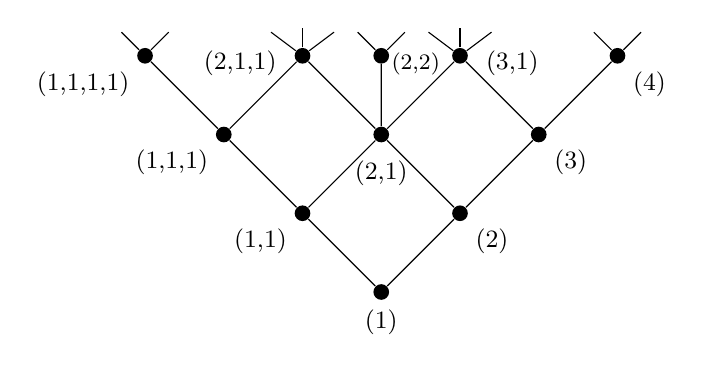
\begin{tikzpicture}[
    dot/.style={circle, fill=black, inner sep=2pt},
    every label/.style={font=\small},
    node distance=12mm and 14mm
]

% level 1 
\node[dot, label=below:{(1)}] (1) at (0,0) {};

% level 2
\node[dot, label=below left:{(1,1)}] (11) at (-1,1) {};
\node[dot, label=below right:{(2)}] (2) at (1,1) {};

% level 3
\node[dot, label=below left:{(1,1,1)}] (111) at (-2,2) {};
\node[dot, label={[yshift=-1mm]below:(2,1)}] (21) at (0,2) {};
\node[dot, label=below right:{(3)}] (3) at (2,2) {};

% level 3
\node[dot, label=below left:{(1,1,1,1)}] (1111) at (-3,3) {};
\node[dot, label={[xshift=-1mm,yshift=-1mm]left:(2,1,1)}] (211) at (-1,3) {};
\node[dot, label={[xshift=-1mm,yshift=-1mm]right:{{\footnotesize(2,2)}}}] (22) at (0,3) {};
\node[dot, label={[xshift=1mm,yshift=-1mm]right:(3,1)}] (31) at (1,3) {};
\node[dot, label=below right:{(4)}] (4) at (3,3) {};

\draw (1)--(11) (1)--(2);
\draw (11)--(111) (11)--(21);
\draw (2)--(21) (2)--(3);
\draw (111)--(1111) (111)--(211);
\draw (21)--(211) (21)--(22) (21)--(31);
\draw (3)--(31) (3)--(4);

% stubs for next level
% (1111) – two stubs
\draw (1111) -- ++(-0.3,0.3);
\draw (1111) -- ++(0.3,0.3);

% (211) – three stubs
\draw (211) -- ++(-0.4,0.3);
\draw (211) -- ++(0,0.35);
\draw (211) -- ++(0.4,0.3);

% (22) – two stubs
\draw (22) -- ++(-0.3,0.3);
\draw (22) -- ++(0.3,0.3);

% (31) – three stubs
\draw (31) -- ++(-0.4,0.3);
\draw (31) -- ++(0,0.35);
\draw (31) -- ++(0.4,0.3);

% (4) – two stubs
\draw (4) -- ++(-0.3,0.3);
\draw (4) -- ++(0.3,0.3);
\end{tikzpicture}
\]

\begin{definition}
    \label{def:poset}
    Το ζεύγος $(P,\leq)$, όπου $P$ είναι σύνολο και $\leq : P\times P \to P$ είναι μια σχέση η οποία είναι 
    \begin{itemize}
        \item \emph{αυτοπαθής}, δηλαδή $x \le x$
        \item \emph{αντισυμμετρική}, δηλαδή αν $x \le y$ και $y \le x$, τότε $x = y$
        \item \emph{μεταβατική}, δηλαδή αν $x \le y$ και $y \le z$, τότε $x \leq z$
    \end{itemize}
    για κάθε $x, y, z \in P$ ονομάζεται \defn{μερική διάταξη} (poset\footnote{Συντομογραφία του {\bf p}artially {\bf o}rdered {\bf set}.}).
\end{definition}

Ένα ακόμα παράδειγμα μερικής διάταξης είναι το ζεύγος $(2^{[n]},\subseteq)$, όπου $2^{[n]}$ είναι το σύνολο όλων των υποσυνόλων του $[n]$, η οποία ονομάζεται \defn{διάταξη Boole}. Για παράδειγμα, 
\[
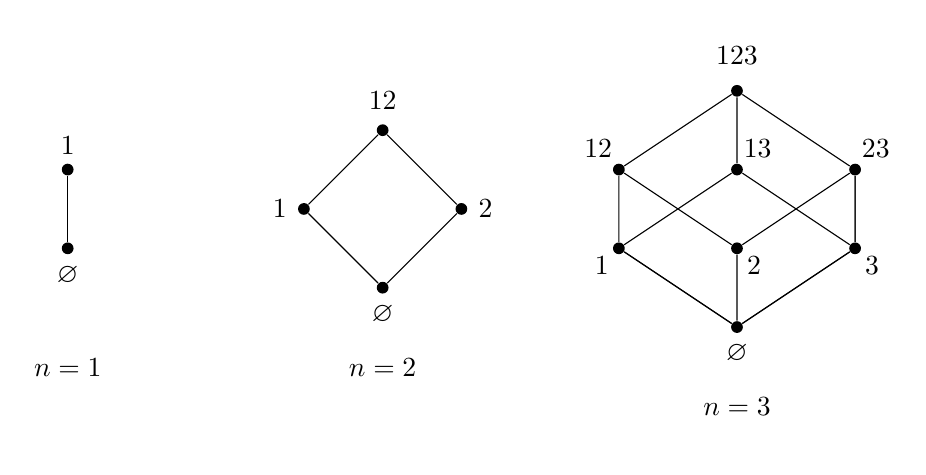
\begin{tikzpicture}[every node/.style={circle, fill, inner sep=1.5pt}]
    \begin{scope}[shift={(0,0.5)}]
    
    \node[label=above:{$1$}] (b) at (0,.5) {};
    \node[label=below:{$\emptyset$}] (a) at (0,-0.5) {};
    \node[below=0.5cm,fill=none] at (0,-1) {$n=1$};

    \draw (a) -- (b);
    \end{scope}

    \begin{scope}[shift={(3,.5)}] 
    \node[label=above:{$12$}] (12) at (1,1) {};
    \node[label=left:{$1$}] (1) at (0,0) {};
    \node[label=right:{$2$}] (2) at (2,0) {};
    \node[label=below:{$\emptyset$}] (0) at (1,-1) {};
    \node[below=0.5cm,fill=none] at (1,-1) {$n=2$};

    \draw (12) -- (1);
    \draw (12) -- (2);
    \draw (1) -- (0);
    \draw (2) -- (0);
    \end{scope}

    \begin{scope}[shift={(7,0)}] 
        \node[label=below left:{$1$}] (a1) at (0,0) {};
        \node[label=below right:{$2$}] (b1) at (1.5,0) {};
        \node[label=below right:{$3$}] (c1) at (3,0) {};
        \node[label=above left:{$12$}] (ab1) at (0,1) {};
        \node[label=above right:{$13$}] (ac1) at (1.5,1) {};
        \node[label=above right:{$23$}] (bc1) at (3,1) {};
        \node[label=above:{$123$}] (abc1) at (1.5,2) {};
        \node[label=below:{$\emptyset$}] (ee1) at (1.5,-1) {};
        \node[below=0.5cm,fill=none] at (1.5,-1) {$n=3$};

        \draw (abc1) -- (ab1) -- (a1) -- (ee1);
        \draw (abc1) -- (bc1) -- (c1) -- (ee1);
        \draw (abc1) -- (ac1) -- (a1) -- (ee1);
        \draw (ab1) -- (b1) -- (ee1);
        \draw (ac1) -- (c1);
        \draw (bc1) -- (b1);
        \draw (bc1) -- (c1) -- (ee1);
    \end{scope}
\end{tikzpicture}
\]

\begin{definition}
    \label{def:composition}
    Μια ακολουθία $\alpha = (\alpha_1, \alpha_2, \dots, \alpha_k)$ θετικών ακεραίων τέτοια ώστε 
    \[
    \alpha_1 + \alpha_2 + \cdots + \alpha_k = n
    \]
    ονομάζεται \defn{σύνθεση} (composition) του $n$. Συμβολίζουμε με $\Comp(n)$ το σύνολο όλων των συνθέσεων του $n$.
\end{definition}

Για παράδειγμα, οι συνθέσεις του $n=3$ είναι 
\[
(1,1,1), \ (1,2), \ (2,1), \ (3).
\]
Σε αντίθεση με τις διαμερίσεις, το πλήθος των συνθέσεων υπολογίζεται αρκετά εύκολα.
\begin{proposition}
    \label{prop:comp_to_set}
    Η απεικόνιση $\rmset: \Comp(n) \to 2^{[n-1]}$ που ορίζεται θέτοντας 
    \[
    \rmset(\alpha) \coloneqq \{\alpha_1, \alpha_1 + \alpha_2, \dots, \alpha_1 + \cdots + \alpha_{k-1}\}
    \]
    για κάθε $\alpha = (\alpha_1, \alpha_2, \dots, \alpha_k) \in \Comp(n)$ είναι αμφιμονοσήμαντη. Ειδικότερα, 
    \[
    \abs{\Comp(n)} = 2^{n-1}.
    \]
\end{proposition}
\begin{proof}[Απόδειξη]
    Θεωρούμε την απεικόνιση $\comp: 2^{[n-1]} \to \Comp(n)$ που ορίζεται θέτοντας 
    \[
    \comp(S) \coloneqq \left(s_1, s_2-s_1, \dots, s_{k}-s_{k-1}, n-s_k\right)
    \]
    όπου $S = \{s_1, s_2, \dots, s_k\} \subseteq [n-1]$ έτσι ώστε $s_1 < s_2 < \cdots < s_k$. Για παράδειγμα, 
    \[
    \renewcommand{\arraystretch}{1.2}
    \begin{array}{c|c|c|c|c|c|c|c|c}
        S        & \emptyset & 1     & 2     & 3     & 12         & 13      & 23      & 123 \\\hline
        \comp(S) & (4)       & (1,3) & (2,2) & (3,1) & 
        (1,1,2)    & (1,2,1) & (2,1,1) & (1,1,1,1)
    \end{array}
    \]
    Η απεικόνιση $\comp$ είναι η αντίστροφη της $\rmset$ (γιατί;) και το ζητούμενο έπεται.
\end{proof}

\newpage

\setcounter{section}{10}
\setcounter{theorem}{0}
\begin{center}
    \textbf{10. Πρότυπα Young
}
\end{center}

Στο Πόρισμα~9.4 είδαμε ότι το σύνολο των ανάγωγων χαρακτήρων της $\fS_n$ παραμετρικοποι\-είται από τις διαμερίσεις του $n$. Στόχος μας στις επόμενες παραγράφους είναι δοθείσης μια διαμέρισης $\lambda \vdash n$, να κατασκευάσουμε ένα ανάγωγο $\fS_n$-πρότυπο $\sS^\lambda$, έτσι ώστε το 
\[
\{\sS^\lambda : \lambda \vdash n\}
\]
να αποτελεί ένα σύνολο ανά δύο μη ισόμορφων ανάγωγων $\fS_n$-προτύπων.

Παρόλο που δεν υπάρχει κάποιος προφανής τρόπος να γίνει αυτό, μπορούμε, ξεκινώντας από μια διαμέριση $\lambda$ της $n$, να κατασκευάσουμε μια υποομάδα $\fS_{\lambda}$ που της αντιστοιχεί με \textquote{φυσικό} τρόπο και να μελετήσουμε τα πρότυπα της μορφής 
\[
V^\triv\uparrow_{\fS_\lambda}^{\fS_n},
\]
όπου $V^\triv$ είναι το τετριμμένο $\fS_\lambda$-πρότυπο.

\begin{definition}
    \label{def:young_subgroup}
    Έστω $\lambda = (\lambda_1, \lambda_2, \dots, \lambda_k) \vdash n$. Το σύνολο $\fS_\lambda$ όλων των μεταθέσεων της $\fS_n$ που σταθεροποιούν\footnote{Μια μετάθεση $\pi \in \fS_n$ \defn{σταθεροποιεί} το $S \subseteq [n]$ αν $\pi(S) = S$.} τα σύνολα
    \[
    [\lambda_1 + \cdots + \lambda_{i-1}+1, \lambda_1 + \cdots + + \lambda_{i-1} + \lambda_i]
    \]
    για κάθε $1 \le i \le k$, όπου $\lambda_0 \coloneqq 0$ και $[a,b] \coloneqq \{a, a+1, \dots, b\}$ για $a \leq b$ ονομάζεται \defn{υποομάδα Young} που αντιστοιχεί στην $\lambda$.
\end{definition}

Με άλλα λόγια, ένα στοιχείο της $\fS_\lambda$ μεταθέτει μεταξύ τους τους πρώτους $\lambda_1$ αριθμούς, τους επόμενους $\lambda_2$ αριθμούς κ.ο.κ. Για παράδειγμα, αν $n= 5$ και $\lambda = (2,2,1)$, τότε η $\fS_\lambda$ περιέχει όλες τις μεταθέσεις της $\fS_5$ οι οποίες σταθεροποιούν τα σύνολα 
\[
\{1,2\}, \ \{3,4\}, \ \{5\},
\]
και γι αυτό 
\[
\fS_{(2,2,1)} = \{\epsilon, \, \cycle{1,2}, \, \cycle{3,4}, \, \cycle{1,2}\cycle{3,4}\}
\]

\begin{remark}
    Αν $G$ και $H$ είναι δυο ομάδες, τότε το $G \times H$ έχει και αυτό δομή ομάδας θέτοντας 
    \[
    (g,h) \ast (g', h') \coloneqq (gg', hh')
    \]
    για κάθε $g, g' \in G$ και $h, h' \in H$. Η τάξη της ομάδας αυτής ισούται με $\abs{G}\abs{H}$. Ομοίως, αν έχουμε ένα αυθαίρετο (πεπερασμένο) πλήθος ομάδων και θεωρήσουμε το καρτεσιανό τους γινόμενο.
\end{remark}

Με την παρατήρηση αυτή κατά νου, η υποομάδα Young είναι όντως υποομάδα της $\fS_n$, διότι 
\begin{align*}
    \fS_\lambda 
    &\cong \fS([\lambda_1]) \times \fS([\lambda_1+1,\lambda_1+\lambda_2]) \times \cdots \times \fS([\lambda_1 + \cdots + \lambda_{k-1}+1, n]) \\
    &\cong \fS_{\lambda_1} \times \fS_{\lambda_2} \times \cdots \times \fS_{\lambda_k},
\end{align*}
όπου ο δεύτερος ισομορφισμός έπεται από το γεγονός ότι $\fS(S) \cong \fS(T)$ αν και μόνο αν $\abs{S} = \abs{T}$ (γιατί;). Στο τρέχον παράδειγμα,  
\begin{align*}
\fS([1,2]) \times \fS([3,4]) \times \fS([5,5]) 
&= \{12, 21\} \times \{34, 43\} \times \{5\} \\
&= \{(12,34,5), (21,34,5), (12, 43, 5), (21, 43, 5)\} \\
&\cong \{12345, 21345, 12435, 21435\} \\
&= \{\epsilon, \cycle{1,2}, \cycle{3,4}, \cycle{12}\cycle{3,4}\} \\
&= \fS_{(2,2,1)}.
\end{align*}

Όπως θα δούμε παρακάτω, το πρότυπο
\[
V^\triv\uparrow_{\fS_\lambda}^{\fS_n}
\]
έχει μια αρκετά απλή μορφή ως αναπαράσταση μεταθέσεων για μια δράση της συμμετρικής ομάδας στα εξής (συνδυαστικά) αντικείμενα.

\begin{definition}
    \label{def:young_tableau}
    \defn{Young ταμπλώ} (Young tableau), ή απλούστερα ταμπλώ, σχήματος $\lambda \vdash n$ και περιεχομένου $[n]$ ονομάζεται μια αμφιμονοσήμαντη αντιστοιχία μεταξύ του συνόλου των τετραγώνων του διαγράμματος Young της $\lambda$ και του $[n]$.
\end{definition}

Για παράδειγμα, ένα ταμπλώ σχήματος $(4,2,2,1)$ και περιεχομένου $[9]$ είναι 
\[
T = \
\begin{ytableau}
7 & 3 & 8 & 2 \\
1 & 5 \\
4 & 9 \\
6
\end{ytableau}.
\]
Τα ταμπλώ σχήματος $(2,1)$ είναι 
\[
\left\{\,
\begin{ytableau}
    1 & 2 \\
    3
\end{ytableau}\,, \
\begin{ytableau}
    2 & 1 \\
    3
\end{ytableau}\,, \
\begin{ytableau}
    1 & 3 \\
    2
\end{ytableau}\,, \
\begin{ytableau}
    3 & 1 \\
    2
\end{ytableau}\,, \
\begin{ytableau}
    2 & 3 \\
    1
\end{ytableau}\,, \
\begin{ytableau}
    3 & 2 \\
    1
\end{ytableau}\,
\right\}.
\]

Η δράση καθορισμού της $\fS_n$ στο $[n]$ επάγει μια δράση στο σύνολο όλων των ταμπλώ σχήματος $\lambda$ και περιεχομένου $[n]$ με τον προφανή τρόπο. Για παράδειγμα, αν $n=9$, $\lambda = (4,2,2,1)$ και $\pi = \cycle{1,3,9,8}\cycle{2,7,6,5,4} \in \fS_9$, τότε 
\[
\pi T = 
\begin{ytableau}
    6 & 9 & 1 & 7 \\
    3 & 4 \\
    2 & 8 \\
    6
\end{ytableau}\, .
\]

Δοθέντος ενός ταμπλώ $T$, θεωρούμε τις υποομάδες $\rmR(T)$ και $\rmC(T)$ της $\fS_n$ που περιέχουν τις μεταθέσεις που σταθεροποιούν τα στοιχεία των γραμμών και των στηλών του $T$, αντίστοιχα. Στο τρέχον παράδειγμα, 
\begin{align*}
    \rmR(T) 
    &\cong \fS(\{2,3,7,8\}) \times \fS(\{1,5\}) \times \fS(\{4,9\}) \times \fS(\{6\}) \\  
    \rmC(T) 
    &\cong \fS(\{1,4,6,7\}) \times \fS(\{3,5,9\}) \times \fS(\{8\}) \times \fS(\{2\}).\\  
\end{align*}

\begin{definition}
    \label{def:young_tabloid}
    Έστω $T$ ένα ταμπλώ σχήματος $\lambda$. Η τροχιά του $T$ στη δράση της $\rmR(T)$ ονομάζεται \defn{ταμπλοειδές} (tabloid) σχήματος $\lambda$ και συμβολίζεται με $[T]$.
\end{definition}

Με άλλα λόγια, η $[T]$ είναι η κλάση ισοδυναμίας με αντιπρόσωπο το ταμπλώ $T$, όπου δύο ταμπλώ ίδιου σχήματος θεωρούνται ισοδύναμα αν και μόνο αν σε κάθε γραμμή έχουν το ίδιο σύνολο στοιχείων. Για παράδειγμα, υπάρχουν τρία ταμπλοειδή σχήματος $(2,1)$ 
\begin{align*}
    \ytableausetup{tabloids}
    \begin{ytableau}
        1 & 2 \\
        3
    \end{ytableau} \ &= 
    \ytableausetup{notabloids}
    \left\{\,
    \begin{ytableau}
    1 & 2 \\
    3
    \end{ytableau}\,, \
    \begin{ytableau}
    2 & 1 \\
    3
    \end{ytableau}\,
    \right\}
    \\[6pt]
    \ytableausetup{tabloids}
    \begin{ytableau}
        1 & 3 \\
        2
    \end{ytableau} \ &= 
    \ytableausetup{notabloids}
    \left\{\,
    \begin{ytableau}
    1 & 3 \\
    2
    \end{ytableau}\,, \
    \begin{ytableau}
    3 & 1 \\
    2
    \end{ytableau}\,
    \right\}
\\[6pt]
\ytableausetup{tabloids}
    \begin{ytableau}
        2 & 3 \\
        3
    \end{ytableau} \ &= 
    \ytableausetup{notabloids}
    \left\{\,
    \begin{ytableau}
    2 & 3 \\
    1
    \end{ytableau}\,, \
    \begin{ytableau}
    3 & 2 \\
    1
    \end{ytableau}\,
    \right\}.
\end{align*}
Στην πράξη, όταν γράφουμε ένα ταμπλοειδές θα \textquote{ξεχνάμε} τις κάθετες γραμμές στο διάγραμμα Young για να υποδείξουμε ότι μπορούμε ελεύθερα να μεταθέσουμε τα στοιχεία κάθε γραμμής και να προκύψει το ίδιο ταμπλοειδές.

Η παραπάνω δράση της $\fS_n$ στα ταμπλώ περιεχομένου $[n]$ επεκτείνεται και στο σύνολο των ταμπλοειδών περιεχομένου $[n]$ θέτοντας 
\[
\pi \cdot [T] \coloneqq [\pi T]
\]
για κάθε $\pi \in \fS_n$ και κάθε ταμπλώ $T$ περιεχομένου $[n]$. 

Η δράση αυτή είναι καλά ορισμένη. Πράγματι, αν $[T] = [Q]$, τότε, από τον Ορισμό~\ref{def:young_tabloid}, $Q = \pi{T}$ για κάποια $\pi \in \rmR(T)$. Συνεπώς, για κάθε $\sigma \in \fS_n$ έχουμε 
\[
\sigma{Q} = \sigma\pi{T} = (\sigma\pi\sigma^{-1})\sigma{T},
\]
όπου $\sigma\pi\sigma^{-1}\in \rmR(\sigma{T})$ (γιατί;\footnote{Για την ακρίβεια, παρατηρήστε ότι $\rmR(\sigma{T}) = \sigma\rmR(T)\sigma^{-1}$ για κάθε $\sigma \in \fS_n$ και κάθε ταμπλώ $T$ περιεχομένου $[n]$.}) και γι αυτό, πάλι από τον Ορισμό~\ref{def:young_tabloid}, $[\sigma{T}] = [\sigma{Q}]$ ή ισοδύναμα $\sigma\cdot[T] = \sigma\cdot[Q]$, όπως θέλαμε.

\begin{definition}
    \label{def:young_module}
    Η αναπαράσταση μεταθέσεων που επάγεται από τη δράση της $\fS_n$ στο σύνολο όλων των ταμπλοειδών σχήματος $\lambda$ ονομάζεται \defn{πρότυπο Young} (Young module) και συμβολίζεται με $\rmM^\lambda$.
\end{definition}
\end{document}